\begin{frame}
\frametitle{Hardware used in this training session}
  BeagleBone Black, from CircuitCo
  \begin{columns}
    \column{0.65\textwidth}
    \footnotesize
    \begin{itemize}
      \item Texas Instruments AM335x (ARM Cortex-A8 CPU)
      \item SoC with 3D acceleration, additional processors
        (PRUs) and lots of peripherals.
      \item 512 MB of RAM
      \item 4 GB of on-board eMMC storage
      \item Ethernet, USB host and USB device, microSD, micro HDMI
      \item 2 x 46 pins headers, with access to many expansion buses
        (I2C, SPI, UART and more)
      \item A huge number of expansion boards, called {\em capes}.
        See \url{http://elinux.org/Beagleboard:BeagleBone_Capes}.
    \end{itemize}
    \column{0.35\textwidth}
    \begin{center}
      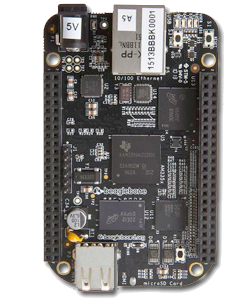
\includegraphics[width=\textwidth]{slides/beagleboneblack-board/beagleboneblack.png}\\
      
\includegraphics[width=0.5\textwidth]{slides/beagleboneblack-board/open-source-hardware-logo.pdf}
    \end{center}
  \end{columns}
\end{frame}

\begin{frame}
\frametitle{Do not damage your BeagleBone Black!}
\begin{itemize}
  \item Do not remove power abruptly:
  \begin{itemize}
     \item Boards components have been damaged by removing the power or
           USB cable in an abrupt way, not leaving the PMIC the time to
           switch off the components in a clean way. See
           \url{http://bit.ly/1FWHNZi}
     \item Reboot (\code{reboot}) or shutdown (\code{halt}) the board
	   in software when Linux is running.
     \item You can also press the \code{RESET} button to reset and
	   reboot.
     \item When there is no software way, you can also switch off
	   the board by pressing the \code{POWER} button for 8 seconds.
  \end{itemize}
  \item Do not leave your board powered on a metallic surface (like a
        laptop with a metal finish).
\end{itemize}
\end{frame}
